%!TEX root = ../Thesis.tex
\chapter{Introduction}
\label{chap:introduction}
In this chapter, we provide an overview of the thesis, which includes its foundational background, the purpose and objectives to be pursued, and the identified problems. Additionally, we point out the thesis's contributions, and structure.

\section{Background}
In contemporary computational science and AI, using HPC systems has become advantageous and indispensable. As the boundaries of human knowledge expand, so do the complexities of the problems we seek to solve. From simulating climate models to analyzing vast datasets in genomics and training deep neural networks to powering advanced simulations in fluid dynamics, HPC emerges as the bedrock for modern scientific research and technological advancement.

Traditional HPC clusters emphasized CPU-centric computing. However, the rise of heterogeneous computing has introduced supercomputers with accelerators such as the GPU \cite{5289128}. At the core of current computational revolution lies the GPU, which has transcended its original purpose in graphics rendering to become the cornerstone of parallel computing. In artificial intelligence, the demand for GPU resources for training has surged dramatically, driven by the increasing complexity of neural network models and the rise of LLMs in recent years. The significance of GPUs in HPC cannot be overstated, as their massively parallel architecture and ability to handle thousands of computational tasks simultaneously have pushed scientific research and AI development to new heights. Indeed, GPUs have redefined the limits of what was once computationally feasible, enabling researchers and engineers to tackle problems of immense scale and complexity with remarkable efficiency and speed.

As a result, effective GPU monitoring has become an indispensable component for ensuring optimal performance, reliability, and resource utilization. Comprehensive monitoring solutions are paramount as computational workloads become increasingly complicated and resource-intensive. GPU monitoring provides invaluable insights into the utilization, temperature, power consumption, and memory usage of GPUs in real-time, enabling researchers and system administrators to identify bottlenecks, preemptively address hardware failures and code bugs, and optimize resource allocation. This proactive approach enhances the overall efficiency and stability of HPC environments, minimizes downtime, and maximizes the return on investment in GPU-accelerated infrastructure.

Furthermore, with the growing popularity of AI applications, from natural language processing to computer vision, the demand for GPU resources continues to grow. Effective monitoring ensures the smooth operation of AI training jobs. It facilitates capacity planning and scalability to ensure that all the resources are used efficiently, allowing HPC users to seamlessly adapt to evolving computational demands. Through the lens of this thesis, we aim to underscore how we conduct GPU monitoring to harness the full potential of HPC in real-world applications, showing its pivotal role in driving innovation, enhancing system performance, and advancing the frontiers of both scientific research and artificial intelligence.

\section{Purpose}
Most workload managers in the HPC world lack a GPU monitoring feature. Implementing a real-time GPU usage alert service at the job level on HPC clusters can yield significant benefits across various domains. Notably, it can enhance the overall sustainability of utilizing the computing cluster while facilitating the advancement of generative AI development.

\subsection{Sustainability}

In HPC environments, GPUs are typically allocated by the device, while the CPU allocates cores. For instance, the LUMI supercomputer, ranked as the fastest in Europe according to TOP500 by June 2024 \cite{TOP500}, uses AMD Radeon Instinct MI250X GPU Accelerator, which is equipped with 220 compute units (cores), in contrast to the 64-core 3rd Gen EPYC 7A53s Trento CPU \cite{lumi}. While this abundance of cores enables GPUs to efficiently handle mathematical and spatial computations simultaneously, it makes GPUs the most power-intensive component in a computing system.

Compared with CPUs, inefficient utilization of GPUs can lead to substantial resource wastage, particularly during peak hours when numerous jobs await allocation. Referring to Subsection \ref{subsec:lumi}, as is shown in Table \ref{tab:lumi_resources}, in LUMI, the maximum TDP for the CPU is 280W \cite{amd-epyc-cpu}, whereas the TBP for the GPU is 500W, peaking at 560W \cite{amd-mi250x}. Thus, each allocation on systems like LUMI has a mere 4W energy consumption per core for CPUs, contrasting wildly with the over 250W consumption for GPUs (1 GPU has 2 GCDs in this case here) \cite{lumi}.

\begin{table}[H]
    \centering
    \begin{tabular}{|c|c|c|c|c|c|}
        \hline
        \textbf{Device} & \textbf{Cores} & \textbf{Maximum Power} & \textbf{Allocable} & \textbf{Allocation Power} \\
        \hline
        \textbf{GPU} & 220 & 560W & 2 & 280W \\
        \hline
        \textbf{CPU} & 64 & 280W & 64 & 4.375W \\
        \hline
    \end{tabular}
    \caption{Resources comparison of GPU and CPU for LUMI}
    \label{tab:lumi_resources}
\end{table}

However, for GPU, knowing the performance and getting alerted for sub-optimal jobs on time poses a challenge for supercomputer administrators. Existing workload managers and job schedulers in HPC systems, such as Slurm and LSF, provide descriptive accounts of CPU and memory usage but lack real-time hardware monitoring capabilities at the job level, and they have no recording of history monitoring data. They also have no built-in alert systems. As a result, a GPU alerting system is urgently needed to help administrators ensure sustainability and reduce carbon emissions. Users also need this information to debug or improve the code and make their programs more environmentally friendly.


\subsection{Generative AI}
In January 2024, the European Commission introduced comprehensive measures to bolster European startups and SMEs (Small and Medium-sized Enterprises) in developing AI that upholds EU values and regulations \cite{eu-ai}. This initiative follows the political consensus reached in December 2023 regarding the EU AI Act, which is tailored to support AI startups and foster innovation. It includes a proposal aimed at amending the Regulation of the EuroHPC JU (European High-Performance Computing Joint Undertaking) \cite{european_union_2021}, thereby granting startups and the broader innovation community access to AI-optimized supercomputers --- AI Factories.

AI Factories leverage the supercomputing capacity of the EuroHPC Joint Undertaking to develop trustworthy, cutting-edge generative AI models. Generative AI, now a trendy research area, focuses on creating new content or data that is original and often indistinguishable from human-created content. These models are trained on vast amounts of text data to learn the intricacies of language. They can then generate coherent and contextually relevant text, pictures, sound, and videos in various styles and topics. Through fine-tuning and conditioning on specific prompts or input contexts (prompt engineering), LLMs can generate text that mimics human writing remarkably, making them valuable tools for various creative and practical applications, including content generation, story writing, and even code generation. Most of the generative AI models, such as LLaMA \cite{touvron2023llama}, Gemma \cite{gemmateam2024gemma} as well as OpenAI's GPT series \cite{openai2024gpt4}, use transformers. 

% \begin{figure}[H]
%     \centering
%     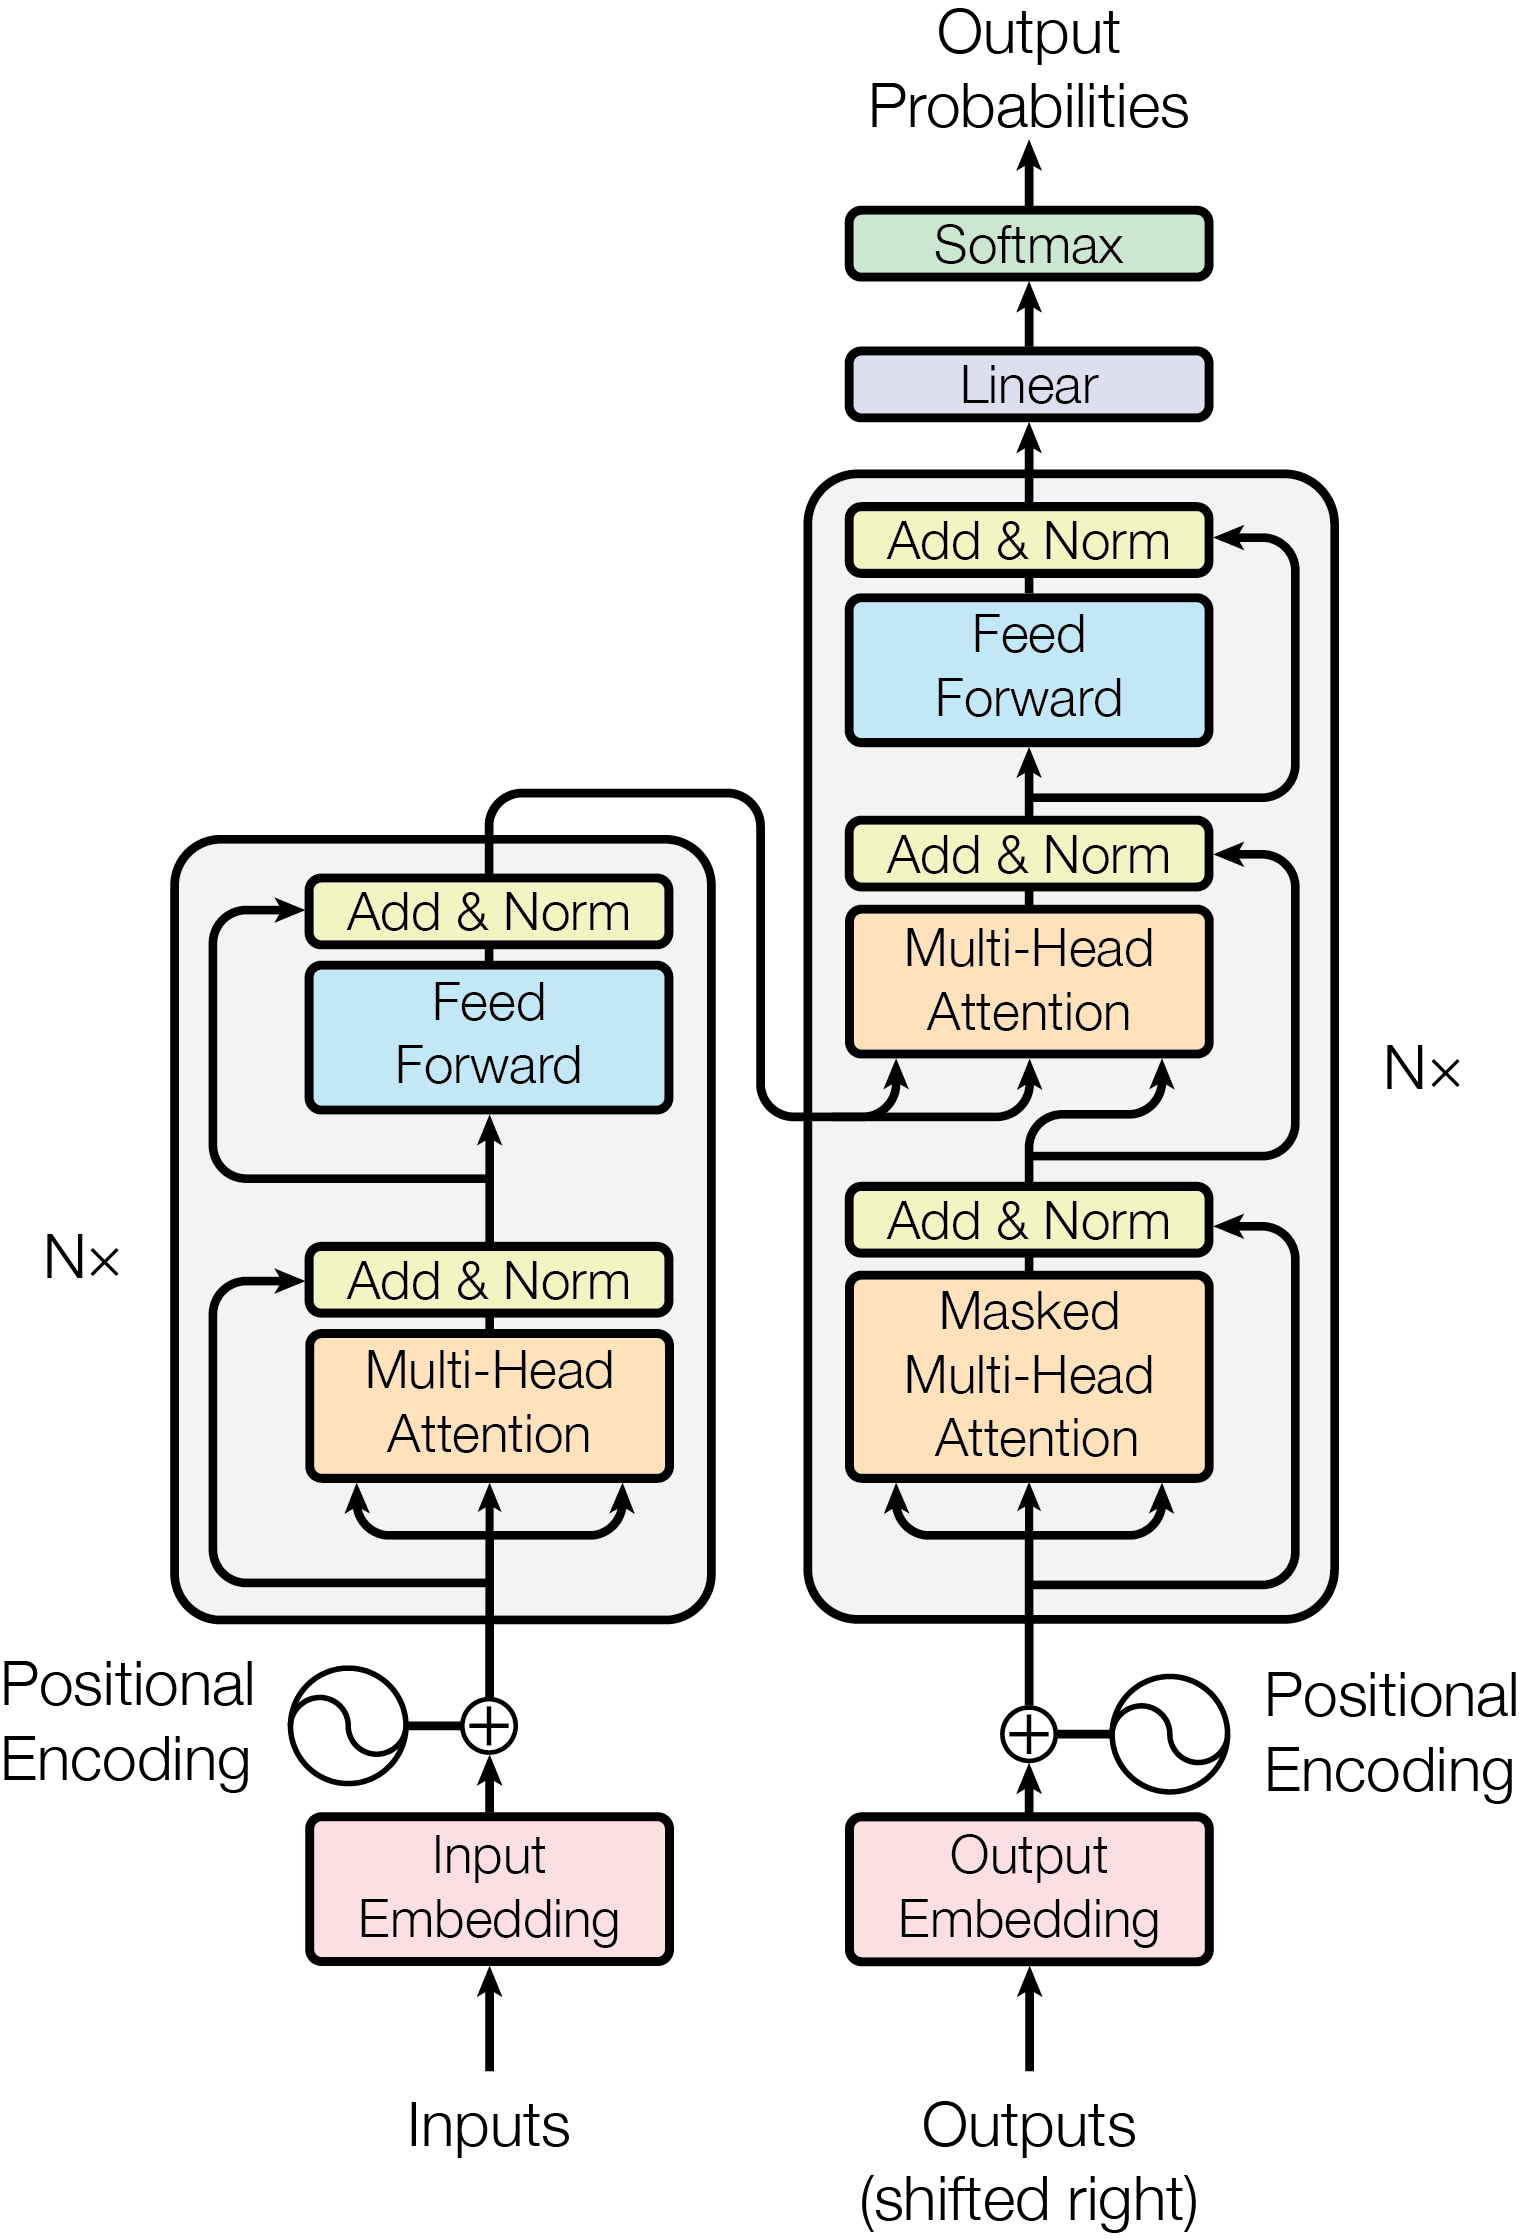
\includegraphics[width=0.6\textwidth]{figures/ModalNet-21.png}
%     \caption{Transformer model architecture \cite{NIPS2017_3f5ee243}}
%     \label{fig_transformers}
% \end{figure}

Transformers employ attention mechanisms to capture dependencies between words in a sequence, allowing them to understand and generate text with greater contextual awareness \cite{NIPS2017_3f5ee243}. The architecture of transformers, characterized by their extensive layers and attention mechanisms, necessitates vast amounts of parallel computation, making them an ideal fit for GPU acceleration.

GPUs excel at handling the matrix multiplications and element-wise operations inherent in the forward and backward passes of transformer models, leveraging their massively parallel architecture to accelerate training and inference processes. Moreover, GPUs' large memory bandwidth helps efficiently process the immense datasets typically associated with LLMs, enabling scalability. As a result, integrating GPUs in LLM frameworks enhances computational performance. It allows researchers and practitioners to explore more complex models and larger datasets, pushing the boundaries of natural language understanding and generation. 

However, due to the highly intensive model structure and the complicated nature of distributed parallel training and inference logic, those generative AI training programs and inference applications will likely not utilize all the GPUs fully. GPU monitoring and alerting can provide insights into the performance and help identify code bugs and optimization opportunities for AI workloads, thus advancing state-of-the-art AI research and applications.

\section{Research questions}
\label{sec:rqs}
By the time we started the thesis, a monitoring system for GPU had already been ready as part of the work during my 2023 summer internship at CSC -- IT Center for Science. As a result, this thesis aims to impact the above areas by implementing an alert service based on our existing monitoring system for supercomputers at CSC. It seeks to address the following research question:

\textbf{
How do we systematically design a service that efficiently and reliably analyzes jobs using GPUs in HPC systems in real-time?
}

This can be divided into the following sub-research questions:

\begin{itemize}
    \item \textbf{RQ1}: \textit{How to minimize the alert delay with a fix-size window in real-time?}

This involves exploring efficient methods to streamline detecting and responding to anomalies or critical events promptly.

    \item \textbf{RQ2}: \textit{How to minimize the performance impact on the database systems?}

This includes optimizing database queries and resource allocation to ensure minimal disruption to overall system performance.

    \item \textbf{RQ3}: \textit{How to reliably maintain a data structure for job alert status check?}

This involves data organization, scalability, and fault tolerance to ensure reliable operation under varying workload conditions.
    
    \item \textbf{RQ4}: \textit{How to find the most reliable algorithm for generating alerts?}

This includes assessing different algorithms' accuracy, efficiency, and scalability to determine their suitability for real-time alert generation for HPC.

\end{itemize}


\section{Contributions}

The contributions of this thesis are as follows:

\begin{itemize}
    \item We have successfully created and deployed the monitoring system and the alert service for Nvidia and AMD GPUs at job level with Slurm on HPC systems.
    \item Through an in-depth investigation of the collected monitoring data, an algorithm has been developed to identify and alert jobs with inefficient GPU resource usage. This achievement not only enhances the effectiveness of the alert service but also contributes to optimizing resource utilization and improving overall system efficiency.
    \item By analyzing the collected monitoring data and identifying patterns of inefficient GPU usage, this thesis contributes to a deeper understanding of resource utilization changes and patterns within HPC environments. This knowledge can inform future research and development efforts to optimize GPU-accelerated computing and improve the performance of AI workloads on HPC.
\end{itemize}

\section{Thesis structure}

In this thesis, we systematically explore techniques and methodologies for designing and implementing a monitoring system and alert service for GPU resource utilization on HPC clusters. Following the introduction, which provides background information, outlines the application domains, and presents research questions and contributions, the thesis is organized as follows:

Chapter \ref{chap:background} focuses on the background, which discusses various techniques for building the monitoring system and the alert service. This includes an examination of job schedulers, an overview of HPC systems at CSC (including Puhti, Mahti, and LUMI), an overview of the time-series database TimescaleDB, as well as an exploration of different monitoring systems techniques, such as /proc, Cgroups, NVML, and ROCm-SMI, database techniques including triggers, LISTEN \& NOTIFY, and continuous aggregates. Additionally, the section delves into alert algorithms, covering descriptive statistics, decision trees, and random forests, K-Means clustering and silhouette analysis.

Chapter \ref{chap:methods} details the methods we use for implementing the system, which include developing a monitoring daemon, timescale ingest, timescale reader, alert service, and alert dashboard, configuring TimescaleDB, and designing alert algorithms.

In Chapter \ref{chap:result}, benchmark results from both experimental and production setups are presented and analyzed. This includes an overview of the experimental setup, benchmarking results, and insights from production environments by case studies.

Chapter \ref{chap:discussion} discusses the findings, analyzing related work and their implications and limitations.

Finally, Chapter \ref{chap:conclusions} provides concluding remarks, including a summary of critical points and suggestions for future work.
